\section{Canonical Manifolds}
We will now focus on networks with a single learnable embedding matrix, matching the setups of \citet{nanda2023progress,zhong2023the,mccracken2025uncoveringuniversalabstractalgorithm}.
Our analysis will center on the \emph{representation manifolds} in a frequency cluster $f$ coming from the preactivations $\preactivationmap{\ell}(a, b)$ at layer $\ell$ and the logits $\logitmap(a, b)$. The corresponding representation manifolds are, explicitly,
\begin{align*}
    \preactivationmanifold{\ell} &:= \left\{\preactivationmap{\ell}(a, b) : (a, b)\in\mathbb{Z}_n^2\right\} \subset \mathbb{R}^{d_{\ell,f}};\quad\mathrm{and}\quad
    \logitmanifold := \left\{\logitmap(a, b) : (a, b)\in\mathbb{Z}_n^2\right\}\subset\mathbb{R}^n,
\end{align*}
where $d_{\ell, f}$ is the number of neuron in the frequency cluster $f$ at layer $\ell$.
Our thesis is that under the simple neuron model of \eqref{eq:simple-neuron-model} introduced by \citet{mccracken2025uncoveringuniversalabstractalgorithm} and a simple application of symmetry corresponding to the interchangeability of $a, b$ in $a + b \mod n$, the exact structure of the $\preactivationmanifold{1}$ manifolds and how they are mapped from inputs $a, b$ can be revealed.
Particularly, we will show that under this model, $\preactivationmanifold{1}$ always encodes the torus $\mathbb{T}^2$ or vector addition disk of Figure \ref{fig:wrapped}---that is, the pizza.

The remainder of this section will proceed by formalizing this result in \S\ref{subsect:theorems}.


\subsection{Simple neuron phase distribution dictates representation manifold}\label{subsect:theorems}
Under the simple neuron model, for any frequency cluster $f$, the only degrees of freedom in the resulting preactivations lie in the maps $(a, b)\mapsto(\phi^L, \phi^R)$ for $a,b\in\mathbb{Z}_n$ learned by neural networks.
Given that modular addition is commutative, one might expect to see a form of symmetry with respect to $\phi^L, \phi^R$.
Particularly, one might expect that $\phi^L\equiv\phi^R$ for all $a, b$ (since swapping the inputs should have no effect on the output), or at the very least that the random variables $\phi^L, \phi^R$ are identically distributed for $A, B\sim\mathrm{Uniform}(\mathbb{Z}_n)$.
It turns out, as we show in the following theorem (whose proof is given in Appendix \ref{section: proofs}), that the resulting manifold $\preactivationmanifold{1}$ takes an easily characterizable form \textit{almost surely} in this event.
We devote \S\ref{sec:results} to validating that the phase maps indeed satisfy these properties in practice---allowing us to easily analyze the geometry of representations across thousands of trained neural networks.

Before stating the theorem, let us introduce some notation that will be useful.
Under the simple neuron model, a neuron indexed $i$ belonging to a neuron cluster with frequency $f$ maps $(a, b)\in\mathbf{Z}_p^2$ to $\cos(\theta_a + \Phi_i^{L}) + \cos(\theta_b + \Phi_i^{R})$, where $\theta_a = 2\pi fa/p$.
The notation $\Phi_i$ is meant to evoke that we model these phases as random variables; these are random due to random initialization and random gradient updates.
The joint distribution of $(\Phi_i^{L}, \Phi_i^{R})$ is denoted $\phasedist{a}{b}\in\Delta([0,2\pi]^2)$.

\begin{theorem}
    \label{thm:disc-torus}
    Let $f\in\mathbf{Z}_p$ for $p\geq 3$, and consider the frequency cluster at layer 1.
    Let $m$ denote the number of neurons in this cluster, and assume $m\geq 2$.
    Define the matrix $X\in\mathbb{R}^{p^2\times m}$ according to $X_{(a, b), i} = \cos(\theta_a + \phi^L_i) + \cos(\theta_b + \phi^R_i)$, denoting the simple neuron preactivations.
    Assume $\phi^L_i, \Phi^{L, b}_i$ are identically distributed for each neuron $i\in\{1,\dots,m\}$ in this cluster, and that the support of $\phasedist{a}{b}$ has positive (Lebesgue) measure. Then the following hold almost surely:
    \begin{enumerate}
        \item\emph{(Perfect phase correlation)} If $\Phi_i^{L, a}$ and $\Phi_i^{R, b}$ are perfectly correlated, in the sense that $\Phi_i^{L, b} \equiv \Phi_i^{R, b}$, then $X$ has a rank-2 factorization $X = V^{\rm disc}W$ with $V^{\rm disc}\in\mathbb{R}^{p^2\times 2}$ satisfying
        \begin{equation}\label{eq:factorization:disc}
            V^{\rm disc}_{(a, b)} = (\cos\theta_a + \cos\theta_b, \sin\theta_a + \sin\theta_b)^\top.
        \end{equation}
        \item\emph{(Phase independence)} Otherwise, $X$ has a rank-4 factorization $X = V^{\rm torus}W$ with $V^{\rm torus}\in\mathbb{R}^{p^2\times 4}$ given by
        \begin{equation}\label{eq:factorization:torus}
            V^{\rm torus}_{(a, b)} = (\cos\theta_a, \sin\theta_a, \cos\theta_b, \sin\theta_b)^\top.
        \end{equation}
    \end{enumerate}
\end{theorem}

Geometrically, the disc can be viewed as a projection of the torus: $(x_1, x_2, x_3, x_4) \mapsto (x_1 + x_3, x_2 + x_4)$. Thus, the torus structure generalizes the vector-addition disc.

Having established this theorem, it is worth stepping back to contextualize its consequences.
As shown by \citet{mccracken2025uncoveringuniversalabstractalgorithm}, first layer preactivations are dominantly simple neurons.
Theorem \ref{thm:disc-torus} shows that, under the symmetry properties of $\Phi_i^{L, a}$ and $\Phi_I^{R, b}$ posited above, the preactivations have simple, low-dimensional structures: in the case of perfect phase correlation, the representation manifold can be compressed to $V^{\rm disc}$, which is precisely the vector addition disc of Figure \ref{fig:wrapped}.
In the case of phase independence, the representation manifold can be compressed to $V^{\rm torus}$, which exactly encodes the torus $\mathbb{T}^2$.

\begin{remark}
    It is noteworthy that the Clock representation from \citet{zhong2023the} \emph{cannot} occur under the hypotheses of Theorem \ref{thm:disc-torus}.
    The remainder of the paper demonstrates that these hypotheses are satisfied empirically with overwhelming probability.
    Thus, while the Clock circuit of \citet{zhong2023the} is theoretically plausible, it does not occur naturally in practice.
    On the other hand, the possibility of the \emph{torus} representation has not previously been identified in the literature.
\end{remark}

A notable consequence of this result is that the geometry and topology of representation manifolds can be characterized by simply investigating the distributions $\phasedist{a}{b}$ of the learned phases.
As we describe in \S\ref{sec:methods}, this can be done quantitatively, allowing us to derive statistical likelihoods of neural circuits arising over thousands of initializations across architectures.



\subsection{Qualitative analysis of intermediate representations}

This section presents the experimental observations that support the predictions of section \ref{subsect:theorems}. Given that learned embeddings are expected to be points on a circle, we consider two MLP-models as simple baselines capturing the closed form of the above manifolds: MLP-Add should add two points on a circle, giving the vector addition disc (Figure~\ref{fig:wrapped}) and MLP-Concat should concatenate two points on a circle, giving the torus $\mathbb{T}^2$. 

In all networks, we cluster neurons together and study the entire cluster at once. This is done by constructing an $n\times n$ matrix, with the value in entry $(a, b)$ corresponding to the preactivation value on datum $(a,b)$.
A 2D Discrete Fourier Transform (DFT) of the matrix gives the key frequency $f$ for the neuron.
The cluster of preactivations of all neurons with key frequency $f$ is the $n^2 \times |$cluster $f|$ matrix, made by flattening each neurons preactivation matrix and stacking the resulting vector for every neuron with the same key frequency. We call this matrix the neuron-cluster of preactivations matrix.

\paragraph{\textbf{Principal component analysis (PCA).}} 
To probe the representational geometry of the first-layer neurons, we perform PCA on the neuron-cluster matrix of pre-activations. This layer is where differences between Clock and Pizza architectures are expected to emerge, since their outputs diverge only after attention. 

Figure~\ref{fig:pca-representations} shows the PCA embeddings for MLP-Add, MLP-Concat, Pizza, and Clock models. Each input pair $(a,b)$ has been remapped following \citep{mccracken2025uncoveringuniversalabstractalgorithm} and coloured by $a+b \bmod n$, so that points close with respect to the modular addition task are visually grouped. 

The results align strikingly with the predictions of Theorem~\ref{thm:disc-torus}. For MLP-Add, Pizza, and Clock, the first two principal components explain more than 99\% of the variance, yielding a 2D disc-like structure (matching the vector addition geometry of Figure~\ref{fig:wrapped}). For MLP-Concat, the first four principal components each explain about 25\% of the variance, producing a toroidal structure.  

Surprisingly, the Clock network—never previously described as having a “pizza disc” exhibits the same 2D disc structure as Pizza and MLP-Add.

\begin{figure}
    \centering
    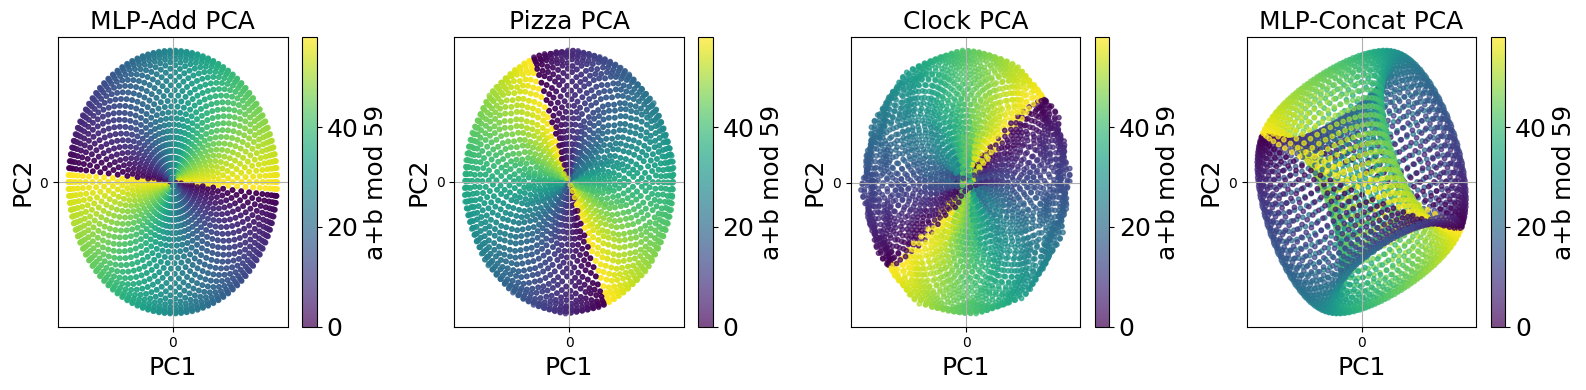
\includegraphics[width=0.9\linewidth]{figures/pca-all-big.png}
    \caption{PCA of neuron pre-activations for a single frequency cluster across architectures: MLP-Add ($f=27$), Pizza ($f=17$), Clock ($f=21$), MLP-Concat ($f=22$). Each point is an input $(a,b)$, colored by $(d\cdot a + d\cdot b)\bmod 59$ corresponding to the network's output (see Section~\ref{sec:prev-interps}). Pizza and Clock are nearly identical to each other and to MLP-Add, but differ strongly from MLP-Concat. Note that the trained pizza and clock models being PCA'd are downloaded directly from \cite{zhong2023the}'s Github: model\_p99zdpze5l.pt and model\_l8k1hzciux.pt.}
    \label{fig:pca-representations}
\end{figure}


\paragraph{\textbf{Distribution of post-ReLU activations.}} 
We next examine the strength of activations across neurons within a cluster. For each neuron, we construct an $n \times n$ heatmap of its post-ReLU activation values over all input pairs $(a,b)$, after applying the remapping procedure of \citep{mccracken2025uncoveringuniversalabstractalgorithm}. Each heatmap thus reflects the activation profile of a single neuron across the input space.  

To summarize activation patterns at the cluster level, we sum the heatmaps of all neurons in the cluster. Although the network never performs this sum directly, it provides a compact visualization of where activation strength is concentrated across the input domain.  

Figure~\ref{fig:sum-postactivations} shows that in MLP-Add, Clock, and Pizza, activations are sharply concentrated along the $a=b$ diagonal. This indicates that cosine responses peak when $a=b$, consistent with neurons having equal phases. Moreover, the smooth falloff of activations away from the diagonal implies that representations also encode the distance $|a-b|$. Because downstream weights from neurons to logits are fixed across inputs, this structure implies that logits systematically depend both on $(a,b)$ and on the separation $a-b$.  

Surprisingly, this diagonal dependence—previously claimed by \cite{zhong2023the} to be the defining characteristic of Pizza—appears not only in Pizza networks but also in MLP-Add and Clock. We return to this point in the experiments section.


\begin{figure}
    \centering
    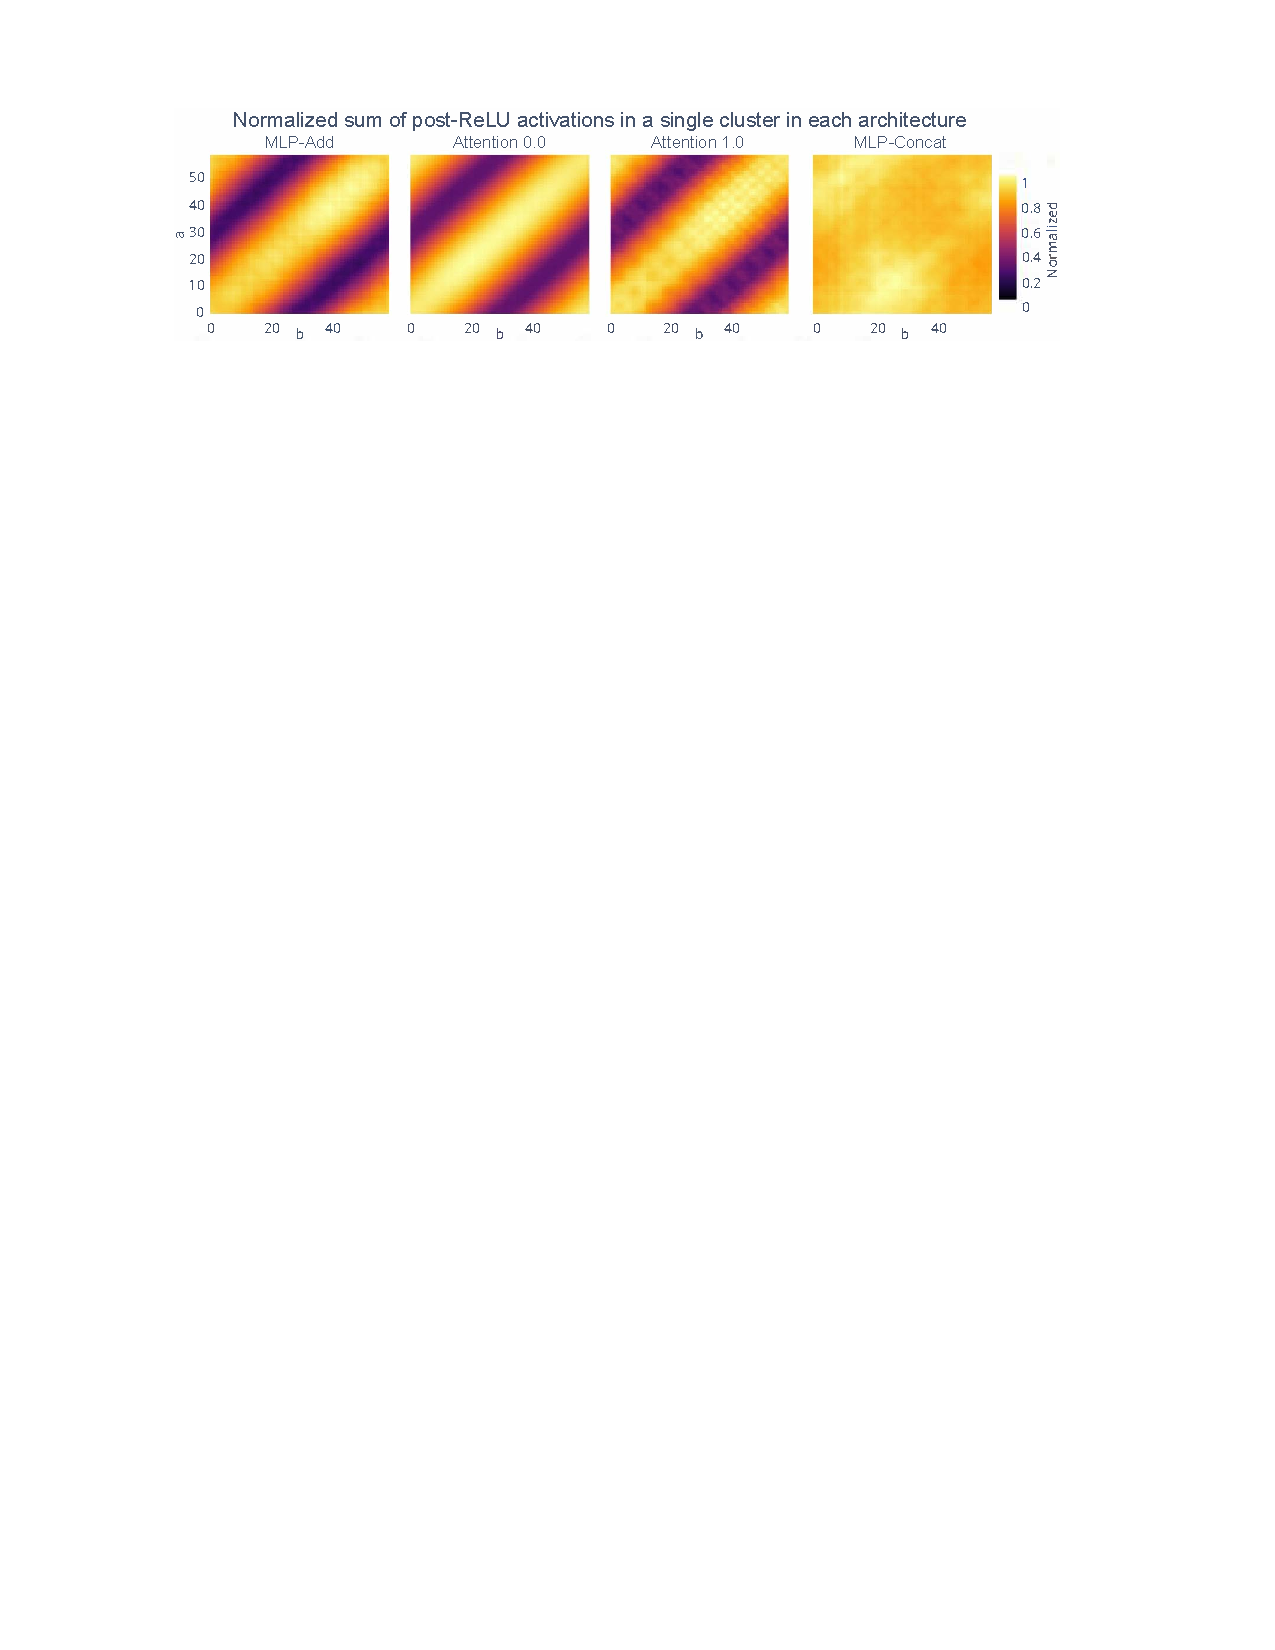
\includegraphics[width=0.9\linewidth]{figures/test_summed.pdf}
    \caption{MLP-Add(f=27), Pizza(f=17), Clock(f=21), MLP-Concat(f=22). Normalized sum of post-activations in clusters in each architecture over all $(a,b)$. Clusters in MLP vector add, Attention 0.0 and 1.0 activate strongest on $(a,b)$ with $a$ close to $b$: the activation strength decreases with distance from $a=b$. Clusters in MLP-Concat activate almost equivariantly.}
    \label{fig:sum-postactivations}
\end{figure}


\paragraph{\textbf{Linking PCA geometry and activation distributions.}} 
The PCA results and activation heatmaps reflect the same underlying phenomenon: principal components encode activation strength. In Figure~\ref{fig:pca-representations}, MLP-Add, Pizza, and Clock show negligible activation near the origin $(0,0)$ of the PCA plane, since neither principal component contributes strongly there. By contrast, for MLP-Concat the 4D embedding contains no datapoints near $(0,0,0,0)$, indicating that the cluster activates roughly equally across all inputs. This observation supports the view that the torus-to-circle map is the natural map for MLP-Concat (Appendix~\ref{app:hypothesis}).

More generally, these findings suggest that activation strength determines how inputs are arranged in PCA space. For MLP-Add, Pizza, and Clock, the dependence on $a-b$ produces an annular geometry at the logits rather than a perfect circle (Figure~\ref{fig:topology-mapping}). For MLP-Concat, the absence of $a-b$ dependence yields a representation closer to a true circle, consistent with the circular structure given in the torus-to-circle map (Appendix~\ref{app:hypothesis}) and illustrated in Figure~\ref{fig:wrapped}. Figure~\ref{fig:topology-mapping} confirms this distinction: MLP-Concat exhibits a torus with a nearly uniform circular projection, while MLP-Add, Pizza, and Clock exhibit a vector addition disc (pizza) with an annular structure at the logits.% (closed form expression in Appendix~\ref{app:annulus}).

Finally, Figure~\ref{fig:topology-mapping} shows the possible manifolds we see in networks across layers.

\begin{figure}
    \centering
    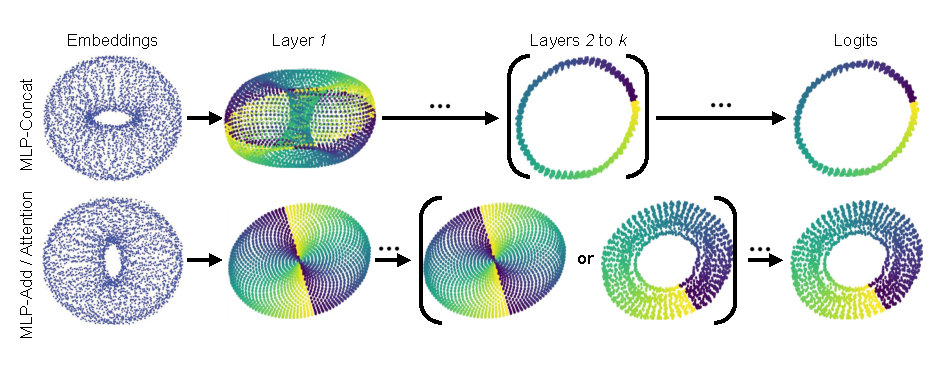
\includegraphics[width=0.9\linewidth]{figures/diagram_final.pdf}
    \caption{Different factorizations of the torus-to-circle map. We find first-layer intermediate representations to be either a torus or a disc (resembling vector addition on the circle). Later layers can construct a circle, and the logits approximate a circle. See Appendix~\ref{app:hypothesis} regarding the torus-to-circle factorization.}
    \label{fig:topology-mapping}
\end{figure}
